\chapter{Marco te\'orico}
\label{cap:marco}
En este capítulo se exponen los conceptos teóricos del presente trabajo de tesis. Primero se explica qué es un motor de búsqueda vertical. Luego se definen las estrategias de evaluación de transacciones de lectura, también conocidas como consultas o \textit{queries}. Posteriormente se describen las diferentes operaciones sobre listas invertidas. Finalmente se explica el concepto de \textit{ranking}. 

\section{Motores de búsqueda verticales}
\label{marco:mbv}
Un motor de búsqueda está construído por diversos componentes, su arquitectura típica se puede ver en la Figura \ref{fig:searchenginearchitecture}. Existe un proceso denominado \textit{crawling}, éste posee una tabla con los documentos iniciales en los que se extrae el contenido de cada uno de ellos. A medida que el \textit{crawler} comienza a encontrar enlaces a otros documentos, la tabla de documentos a visitar crece. El contenido que se extrae en el procedimiento de \textit{crawling} es enviado al proceso de indexamiento, este se encarga de crear un índice de los documentos ya visitados por el \textit{crawler} \citep{Croft:2009}.

\begin{figure}[!th]
\centering
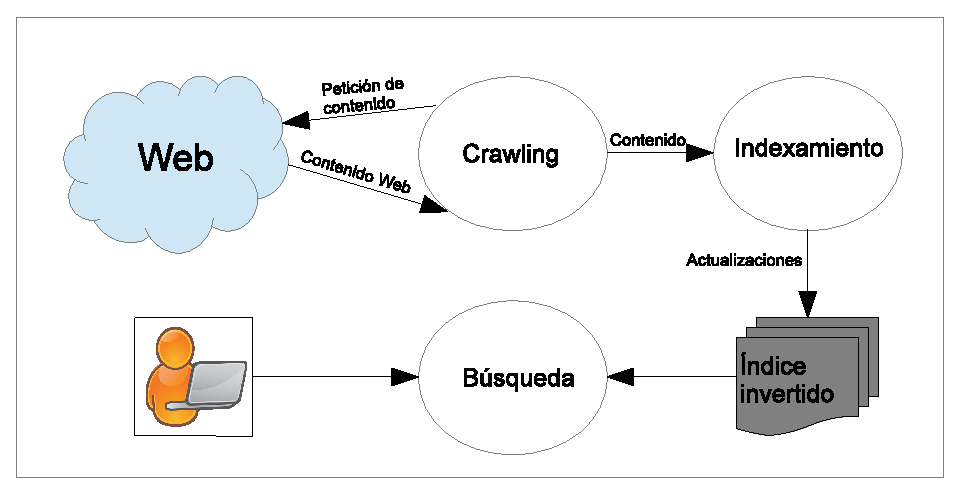
\includegraphics[scale=.75]{images/searchenginearchitecture.eps}
\caption{Arquitectura típica de un motor de búsqueda}
\label{fig:searchenginearchitecture}
\end{figure}

Dado el volúmen de datos involucrado en el procesamiento, se debe tener una estructura de datos que permita encontrar cuáles documentos contienen las palabras presentes en la búsqueda que llega al sistema. Todo esto dentro de un período de tiempo aceptable. El índice invertido \citep{Zobel:2006} es una estructura de datos que contiene un diccionario con todas las palabras que el proceso de \textit{crawling} ha encontrado, asociado a cada palabra se tiene una lista de todos los documentos en donde esta palabra aparece mencionada (conocida como lista invertida de un término). El motor de búsqueda construye esta estructura con el objetivo de acelerar el proceso de las búsquedas que llegan al sistema. El proceso de búsqueda es el encargado de recibir las transacciones de lectura, generar un \textit{ranking} de los documentos que contienen las palabras de la consulta y finalmente generar una respuesta. Las diversas formas de calcular la relevancia de un documento será explicado en secciones posteriores.

En un motor de búsqueda se pueden encontrar diversos servicios tales como (a) cálculo de los mejores documentos para una cierta consulta; (b) construcción de la página Web en la que se mostrará al usuario los resultados; (c) publicidad relacionada con las transacciones de lectura; (d) sugerencias en el momento que el usuario está escribiendo la consulta en el sistema; entre muchos otros servicios.

En los sistemas de recuperación de información como los motores de búsqueda, lo que se hace hoy en día es agrupar computadores para procesar una transacción y obtener la respuesta para ésta. Este conjunto de computadores recibe el nombre de \textit{cluster} \citep{Dean:2009}.

La diferencia entre un motor de búsqueda vertical y uno general, es que el primero se centra solo en un contenido específico de la Web \citep{Gil-Costa:2013}. El \textit{crawler} debe extraer contenido solo de aquellas páginas Web que están dentro del dominio permitido. Al ser un dominio acotado, los documentos a procesar serán menos y por lo tanto, la lista de los términos del índice invertido serán eventualmente de menor tamaño. Sin embargo, en un motor de búsqueda vertical las actualizaciones al índice invertido ocurren con mayor frecuencia.

\section{\'Indice invertido}
\label{marco:ii}
Es una estructura de datos que contiene todos los términos (palabras) encontrados por el \textit{crawler}. A cada uno de los términos está asociado una lista invertida de documentos (páginas Web) que contienen dicho término. Adicionalmente, se almacena información que permita realizar el \textit{ranking} de documentos para generar la respuesta a las consultas que llegan al sistema, por ejemplo, el número de veces que aparece el término en el documento.

Para construir un índice invertido \citep{Baeza-Yates:2011, Salton:2003} se debe procesar cada palabra que existe en un documento, registrando su posición y la cantidad de veces que éste se repite. Cuando se procesa el término con la información asociada correspondiente, se almacena en el índice invertido (ver Figura \ref{fig:invertedindex}).

\begin{figure}[!th]
\centering
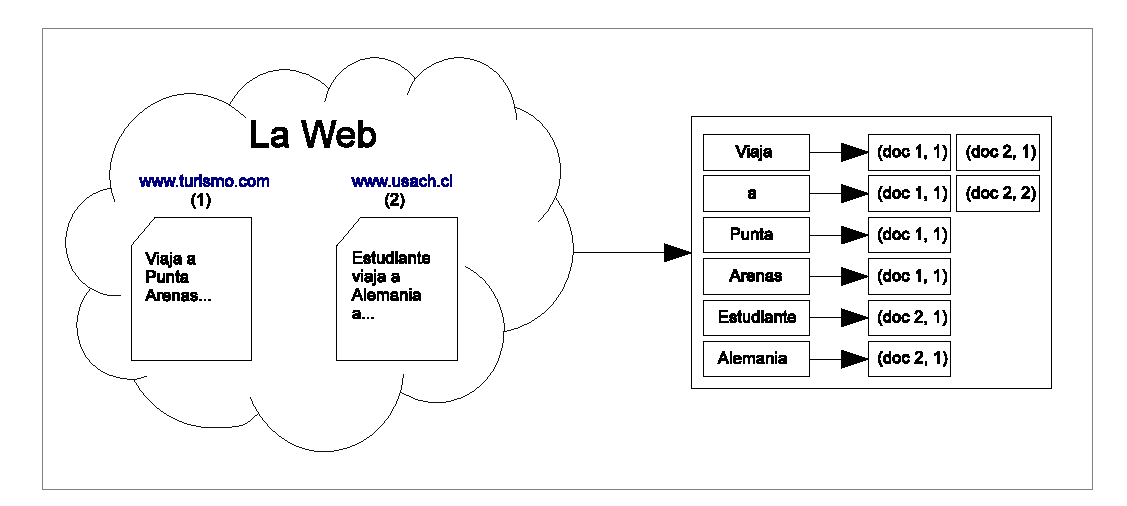
\includegraphics[scale=.75]{images/invertedindex.eps}
\caption{\'Indice invertido}
\label{fig:invertedindex}
\end{figure}

El tamaño del índice invertido crece rápido y eventualmente la memoria RAM se agota antes de procesar toda la colección de documentos. Cuando la memoria RAM se agota, se almacena en disco el índice parcial, se libera la memoria y se continúa con el proceso. Además, se debe hacer un \textit{merge} de los índices parciales uniéndo las listas invertidas de cada uno de los términos involucrados. Es por esto que se han desarrollado algunas técnicas de compresión con el objetivo de guardar de una manera más eficiente el índice invertido \citep{Arroyuelo:2013, Baeza-Yates:2011, Yan:2009}.

\section{Estrategias de evaluaci\'on de transacciones de lectura}
\label{marco:eeq}
Una de las tareas que un motor de búsqueda debe hacer para resolver una consulta es calcular el puntaje o \textit{score} para aquellos documentos relevantes en la consulta y así poder extraer los mejores $K$ documentos. Existen dos principales estrategias para recorrer las listas invertidas y calcular el puntaje de los documentos para una determinada consulta. Estas son (a) \textit{term-at-a-time} \citep{Buckley:1985, Turtle:1995} y (b) \textit{document-at-a-time} \citep{Broder:2003, Turtle:1995}.

\subsection{Term at a time}
Abreviada TAAT, este tipo de estrategia procesa los términos de las consultas una a una y acumula el puntaje parcial de los documentos. Las listas invertidas asociadas a un término son procesadas secuencialmente, esto significa que todos los documentos presentes en la lista invertida del término $t_{i}$ obtienen un puntaje parcial antes de comenzar el procesamiento del término $t_{i+1}$. La secuencialidad en este caso es con respecto a los términos contenidos en la transacción de lectura.

\subsection{Document at a time}
Abreviada DAAT, en este tipo de estrategias se evalúa la contribución de todos los términos de la transacción de lectura con respecto a un documento antes de evaluar el siguiente documento. Las listas invertidas de cada término de la consulta son procesadas en paralelo, de modo que el puntaje del documento $d_{j}$ se calcula considerando todos los términos de la transacción de lectura al mismo tiempo. Una vez que se obtiene el puntaje del documento $d_{j}$ para la consulta completa, se procede al procesamiento del documento $d_{j+1}$. Este tipo de estrategia posee dos grandes ventajas: (a) Requieren menor cantidad de memoria para su ejecución, ya que el puntaje parcial por documento no necesita ser guardado y (b) Explotan el paralismo de entrada y salida (I/O) más eficientemente procesando las listas invertidas en diferentes discos simultáneamente.

\section{Funciones de \textit{Ranking}}
\label{marco:ranking}
Los sistemas de recuperación de información como los motores de búsqueda deben ejecutar un proceso el cual asigna puntaje a documentos con respecto a una determinada transacción de lectura, este proceso se denomina \textit{ranking} \citep{Baeza-Yates:2011}. Como se puede ver en la Figura \ref{fig:ranking_process}, este proceso toma como entrada la representación de las consultas y documentos, y asigna un \textit{score} a un documento $d_{j}$ dada una consulta $q_{i}$.

Un motor de búsqueda guarda billones de documentos que están formados por términos o palabras, estos términos no todos poseen la misma utilidad para describir el contenido del documento. Determinar la importancia de una palabra en un documento no es tarea sencilla, para ello se asocia un peso positivo $w_{i,j}$ a cada término $t_{i}$ del documento $d_{j}$. De esta forma, para un término $t_{i}$ que no aparezca en el documento $d_{j}$ se tendrá $w_{i,j} = 0$. La asignación de pesos a los términos permite generar un \textit{ranking} numérico para cada documento en la colección.

\begin{figure}[!th]
\centering
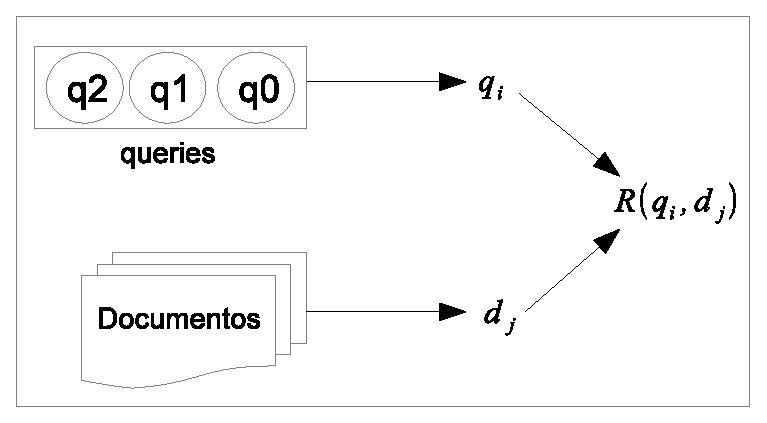
\includegraphics[scale=.75]{images/ranking_process.eps}
\caption{Proceso de \textit{scoring} de documento}
\label{fig:ranking_process}
\end{figure}

\subsection{TF-IDF}
\label{marco:tfi-df}
$Tf-idf$ (\textit{term frequency - inverse document frequency}) es un estadístico que tiene por objetivo reflejar cuán importante es una palabra para un documento en una colección o corpus %. Este estadístico se divide en dos partes, el primero corresponde a la frecuencia del término en un documento ($tf$) y que en su versión más sencilla se utiliza la frecuencia bruta del término $t$ en el documento $d$ ($f(t,d)$) dividido por la frecuencia de la palabra que más se repite en el documento $d$.  

\begin{equation}
\label{formula:tf}
tf(t,d) = \dfrac{f(t,d) }{ \max{f(w,d) : w \in d}}
\end{equation}

El segundo término corresponde a la frecuencia inversa de documento ($idf$) y se utiliza para observar si es que el término es común en el corpus. El $idf$ se obtiene calculando el logaritmo de la división entre el número total de documentos del corpus y el número de documentos que contienen el término.

\begin{equation}
\label{formula:idf}
idf(t,D) = log \frac{ |D| }{1 + |{d \in D : t \in d}|}
\end{equation}

De esta forma a partir de \eqref{formula:tf} y \eqref{formula:idf} se obtiene finalmente el $tf-idf$: 

\begin{equation}
\label{formula:tfi-df}
tf-idf(t,d,D) = tf(t,d) * idf(t,D)
\end{equation}

Notar en \eqref{formula:tfi-df} que el estadístico incrementa proporcionalmente al número de veces que la palabra aparece en el documento, sin embargo, es compensado por la frecuencia de la palabra en la colección completa de documentos o corpus. Esta compensación ayuda a controlar el hecho de que algunas palabras son generalmente más comunes que otras.


\subsection{BM25}
\label{marco:bm25}
Es una función de \textit{ranking} de documentos basada en los términos que aparecen en la consulta que llega al motor de búsqueda. \textit{BM25} pertenece a una amplia gama de funciones de puntuación y está basada en los modelos probabilísticos de recuperación de la información \citep{Baeza-Yates:2011}.

Dada una consulta $Q$ que contiene los términos $q_{1},...,q_{n}$, el \textit{ranking BM25} del documento D se calcula como: 

\begin{equation}
\label{formula:bm25}
score(D,Q) =  \displaystyle\sum_{i=1}^n IDF(q_{i}) * \frac{f(q_{i},D)*(k+1)}{f(q_{i},D)+k * (1 - b + b * \frac{|D|}{prom(docs)})}
\end{equation}

En donde: $f(q_{i}, D)$ es la frecuencia en que aparece el término $q_{i}$ en el documento D; $|D|$ es el número de palabras o términos en el documento D; $prom(docs)$ es la media de número de palabras de los documentos en el corpus; k y b son constantes que depende de las características del corpus en el que se está haciendo la búsqueda, por lo general se asignan los valores de $k = 2$ o $k = 1.2$ y $b = 0.75$; finalmente, $IDF(q_{i})$ es la frecuencia inversa de documento para el término $q_{i}$.


\section{Operaciones sobre listas invertidas}
\label{marco:osli}
Cuando una consulta llega al motor de búsqueda, cada término tiene asociado una lista con todos los documentos en los cuales aparece. El sistema debe decidir qué documentos se analizarán para obtener la respuesta y entregar al usuario una respuesta. A continuación se presenta los modos de operar las listas invertidas para una cierta transacción de lectura.

\subsection{\textit{OR}}
\label{marco:or}
Este operador toma las listas invertidas de cada uno de los términos de la transacción de lectura y ejecuta la disyunción entre ellas. El resultado de este operador es una lista invertida con todos los documentos que contengan al menos un término de la consulta. Finalmente, esta lista invertida se ocupará para obtener los mejores K documentos. Un simple ejemplo se muestra en la Figura \ref{fig:ORoperation}.

\begin{figure}[!th]
\centering
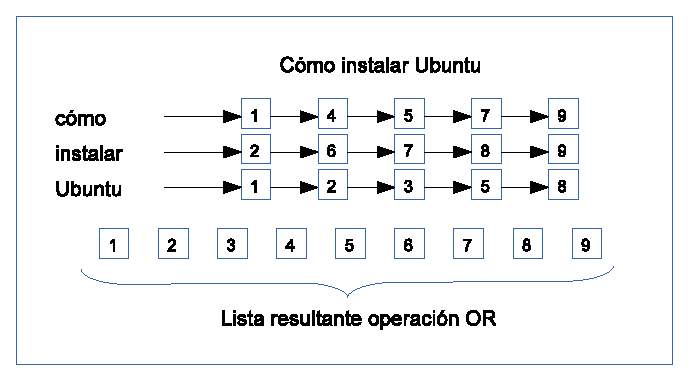
\includegraphics[scale=.75]{images/ORoperation.eps}
\caption{Operaci\'on OR}
\label{fig:ORoperation}
\end{figure}

\subsection{AND}
\label{marco:and}
Este operador ejecuta la conjunción entre las listas invertidas de los términos de una transacción de lectura. Se obtiene una lista invertida con los documentos que contengan todos los términos de la consulta. Se debe notar que aquí se obtiene una lista resultante de menor tamaño que la obtenida en el operador OR (Ver Figura \ref{fig:ANDoperation}).

\begin{figure}[!th]
\centering
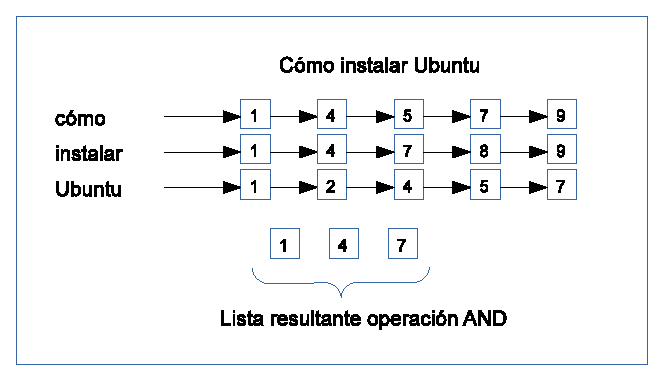
\includegraphics[scale=.75]{images/ANDoperation.eps}
\caption{Operaci\'on AND}
\label{fig:ANDoperation}
\end{figure}

\subsection{Wand}
\label{marco:wand}
Algoritmo de evaluación de transacciones de lectura para obtener eficientemente el conjunto de $K$ documentos que mejor satisfacen una consulta dada. WAND \citep{Broder:2003} es un proceso menos estricto que el método \textit{AND} y está basado en dos niveles. Dentro del proceso de evaluación de una transacción de lectura, uno de los procesos más costoso en términos de tiempo es el de \textit{scoring}, que consiste en entregarle a cada uno de los documentos analizados un puntaje que representa la relevancia del documento para una transacción de lectura dada, esto se denomina evaluación completa o cálculo del puntaje exacto del documento. El objetivo de WAND es minimizar la cantidad de evaluaciones completas de los documentos ejecutando un proceso de dos niveles. En el primer nivel se intenta omitir rápidamente grandes porciones de las listas invertida, lo que se traduce en ignorar el cálculo del puntaje exacto de grandes cantidades de documentos, esto porque en motores de búsqueda a gran escala, este un proceso que requiere de mucho tiempo para llevarse a cabo y depende de factores como la cantidad de ocurrencia del término dentro del documento, el tamaño del documento, entre otros. A este tipo de técnicas que intenta omitir partes de lista invertida se les conoce como técnica de poda dinámica \citep{Broder:2003, Persin:1994, Turtle:1995}. 

Para llevar a cabo el algoritmo WAND y así reducir el número de documentos completamente evaluados durante el proceso de \textit{ranking} de documentos, se necesita calcular los valores estáticos de límite superior (\textit{upper-bounds}), en donde para cada uno de los términos del índice invertido, se toma la lista invertida correspondiente y se extrae el puntaje máximo de contribución de algún documento con respecto al término. El cálculo de los \textit{upper bounds} se lleva a cabo cuando se construye el índice invertido y en donde a cada término del índice se asocia el puntaje máximo que existe en la lista invertida. 

WAND usa un índice invertido ordenado por los identificadores de documentos. En el primer nivel se itera sobre los documentos del índice invertido de cada término y se identifican los potenciales candidatos usando una evaluación aproximada. En el segundo nivel, aquellos documentos candidatos son completamente evaluados y su puntaje exacto es calculado. De esta forma se obtiene el conjunto final de documentos. Se utiliza un heap como estructura de datos para almacenar el conjunto de los mejores $K$ documentos, en donde el elemento superior corresponde al documento con menor puntaje y es el que se utilizará como umbral (\textit{threshold}) para decidir si los siguientes documentos deben ser completamente evaluados o no.

En la Figura \ref{fig:proceso_wand} se puede ver un ejemplo sencillo de cómo el algoritmo Wand trabaja en la resolución de una transacción de lectura de tres términos: 'casa', 'perro' y 'gato'. Como la consulta está compuesta por tres términos, existen tres punteros que recorren cada una de las listas invertidas (notar que cada puntero recorre una lista invertida diferente). Lo primero que se hace es ordenar las listas invertidas de acuerdo a los identificadores de documentos que se están apuntando, razón por la cual en la Figura \ref{fig:proceso_wand} la lista invertida de 'casa' (puntero referenciando al documento con identificador 125), aparece primero que la lista invertida de 'perro' (puntero haciendo referencia al documento con identificador 503). Luego se suma los \textit{uppers bounds} de los términos en orden hasta que se obtiene un valor mayor o igual al \textit{threshold}. De esta manera el término 'perro' es escogido como término pivote ($2.0 + 4.4 \geq 5.7$) y el actual documento al cual se está apuntando es escogido como documento pivote (documento con identificador 503). Si las dos primeras listas invertidas no contienen el documento 503 entonces se procede a seleccionar el siguiente pivote, en otro caso se calcula el puntaje completo del documento. Finalmente, si el puntaje es mayor o igual al \textit{threshold}, se actualiza el \textit{heap} eliminando el elemento superior y se añade el nuevo documento. 
Este algoritmo es repetido hasta que no hayan más documentos a procesar o hasta que no exista un documento que supere el actual \textit{threshold}. De esta manera se evita procesar las listas completas \citep{Blanco:2010}.

\begin{figure}[!th]
\centering
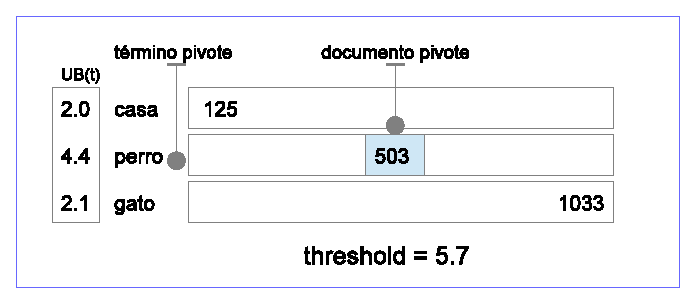
\includegraphics[scale=.75]{images/proceso_wand.eps}
\caption{Ejemplo de ejecución de algoritmo Wand}
\label{fig:proceso_wand}
\end{figure}

\subsection{Block Max Wand}
\label{marco:bmw}
Como se explicó en la sección anterior, la diferencia entre un método exhaustivo de evaluación de documentos y el método Wand, es que este último es una técnica DAAT de poda dinámica \citep{Moffat:1996} en la que se intenta omitir la mayor cantidad de evaluaciones de documentos haciendo uso de una estrategia de movimientos de punteros pivotes.
Bajo la premisa que Wand tradicional es limitado por el hecho que usa los máximos puntajes de las listas invertidas (\textit{Upper bounds}) para podar, puesto que estos pueden ser mucho más grandes que el promedio de puntaje en ellas, se propone un método llamado \textit{Block-Max-Wand} (BMW) \citep{Ding:2011}. Este método utiliza una estructura de datos llamada índice \textit{Block-Max}, en donde el índice invertido estará particionado en bloques y para cada bloque se almacena la máxima contribución de algún documento dentro del bloque. En otras palabras, se tendrán tantos \textit{upper bounds} locales como bloques existan en la lista invertida.

Este método utiliza una variación del algoritmo Wand tradicional para que trabaje correctamente con la nueva estructura \textit{Block-Max-Wand}. Remplazar el uso de los \textit{upper bounds} de cada bloque por el \textit{upper bound} global no garantiza la correctitud del algoritmo. En la Figura \ref{fig:bmw} se muestra un ejemplo de por qué mirar solo los \textit{upper bounds} locales no garantiza obtener los resultados correctos, aquí no se puede concluir que el documento 4868 es el documento más pequeño que puede estar dentro del conjunto \textit{top-K}, ya que $2.5 + 2.0 + 3.5 \geq 7.0$ (conclusión que sí es válida utilizando Wand tradicional y \textit{upper bounds} globales), porque es posible que el bloque siguiente al bloque del docID 275 (en la primera lista), tenga un \textit{upper bound} local mayor. Por lo tanto, aplicar solo las máximas contribuciones por bloque no permite al algoritmo omitir documentos de forma segura.  

\begin{figure}[!th]
\centering
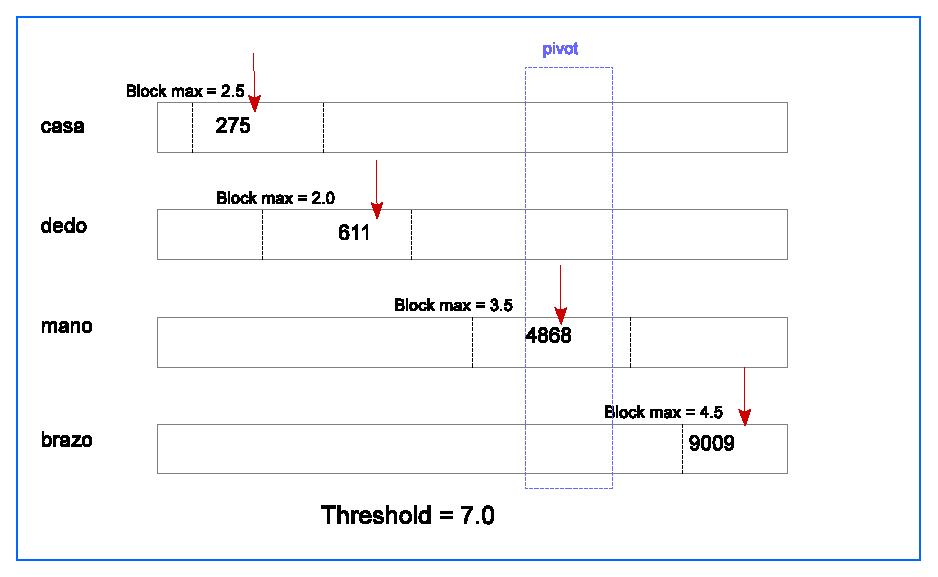
\includegraphics[scale=.75]{images/block-max-wand.eps}
\caption{Ejemplo del proceso \textit{Block-Max-Wand}}
\label{fig:bmw}
\end{figure}

\section{Predicción de tiempo de respuestas de transacciones de lecturas}
\label{marco:prediccion}
El rendimiento (\textit{performance}) de una consulta puede medirse de dos formas: Efectividad y eficiencia. La efectividad tiene relación con la calidad de los documentos extraídos para una cierta consulta y la eficiencia corresponde al tiempo que conlleva procesarla. El tiempo que le toma al sistema en resolver una consulta puede variar considerablemente. Con el objetivo de retornar los resultados al usuario dentro de una cota superior de tiempo, aquellas consultas que toman una mayor cantidad de tiempo en ser procesadas se requiere una mayor cantidad de procesadores para resolverla, de esta forma podemos asegurar esta cota de tiempo. El tener un buen predictor de la eficiencia de una transacción de lectura es muy útil, por ejemplo, si pensamos en un sistema con réplicas, podemos planificar la consulta en el servidor que se desocupará más pronto. 

Existen estudios en los cuales el rendimiento es inferido usando \textit{clarity score} \citep{Cronen-Townsend:2002}, que es una forma para evaluar la pérdida de ambigüedad de una transacción con respecto a la colección. En \citep{He:2004} se propone un conjunto de predictores para el rendimiento de cada consulta. Técnicas de aprendizaje de máquina también han sido estudiadas para predecir el rendimiento de transacciones de lectura \citep{Si:2002}. Todos los estudios mencionados anteriormente se han centrado en la efectividad para ser predicciones de rendimento de transacciones de lectura. La eficiencia de una transacción de lectura también ha sido objeto de estudio, identificando las principales razones que tienen impacto sobre el tiempo de respuesta y evaluando estos factores para predecir el comportamiento de futuras consultas \citep{Tonellotto:2011}. En \citep{Macdonald:2012} se propone un método de predicción de tiempo de respuesta para consultas basado en datos estadísticos disponibles en las respectivas listas invertidas de los términos. Finalmente, en \citep{Jeon:2014} además de utilizar estadísticos disponibles en las listas invertidas de los términos, se agregan estadísticos propios de las consultas para la creación de un predictor. 

\section{Scheduling en motores de búsqueda}
\label{marco:scheduling}
Los motores de búsqueda no solo se preocupan de la calidad de los resultados de las búsquedas (efectividad), sino que también de la velocidad con la que los resultados son obtenidos (eficiencia). Existen varias estrategias para mejorar la velocidad en la obtención de los resultados, una de ellas muy utilizada es el \textit{caching}. Consiste en guardar en memoria de acceso rápido (memoria caché) datos temporales, que luego pueden ser sobrescritos. Una opción es hacer \textit{caching} de los resultados de las búsquedas, de esta forma cuando una consulta es encontrada en caché el motor de búsqueda puede generar la respuesta rápidamente, reduciendo considerablementelos tiempos de calculos. Otra opción es, guardar en caché la intersección de las listas invertidas de pares comunes de términos que llegan al motor de búsqueda. Por ejemplo, si llega al sistema una consulta con los términos ('casa', 'árbol', 'perro'), se puede guardar en caché la intersección de las listas de 'casa' y 'árbol', para luego reutilizar esta información en otras consultas que lleguen en el futuro. Para ver más técnicas de \textit{caching} y ver el detalle de las técnicas mencionadas, ver \citep{Buttcher:2010}. 

Otra estrategia para acelerar el proceso de resolución de transacciones de lectura que llegan al sistema es el uso de algoritmos de planificación (scheduling). Un algoritmo de \textit{scheduling} es el proceso en el cual se cambia el orden en que llegan las consultas al motor de búsqueda con el objetivo de mejorar la eficiencia. 

Existen dos clases de algoritmos de \textit{scheduling}: estáticos y dinámicos. Los estáticos son aquellos en que se conoce el conjunto completo de tareas y las características de cada una de ellas, como por ejemplo, el tiempo de procesamiento. Los algoritmos de \textit{scheduling} dinámicos son aquellos en que no se conoce las tareas que llegarán en el futuro, también se desconoce el momento en que éstas llegarán. La filosofía de los algoritmos de \textit{scheduling} dinámicos es ajustarse a los cambios que pueden haber en el sistema.

En el contexto del presente trabajo de tesis, el objetivo de hacer \textit{scheduling} es minimizar el tiempo en que las consultas son procesadas por un motor de búsqueda. Los motores de búsqueda como \textit{Google}\footnote{http://www.google.com} o \textit{Yahoo!}\footnote{http://www.yahoo.com} trabajan en un contexto \textit{online}. Esto significa que cuando las consultas llegan al sistema (una a una), éste está obligado a tomar una decisión para planificarla sin saber cuáles transacciones de lectura llegarán en un momento posterior. A esto se le conoce como algoritmo de \textit{scheduling online} \citep{Albers:2003, Borodin:1998}.

Los sistemas de recuperación de información a gran escala despliegan una arquitectura distribuída \citep{Dean:2009}, en donde el índice invertido está particionado \citep{Barroso:2003} a lo largo de servidores (\textit{shard servers}), los cuales están encargados de procesar las transacciones de lectura que llegan al sistema. Es fácil notar que resolver una consulta con varios \textit{shard servers} mejoraría la eficiencia. Ahora bien, para asegurar un alto rendimiento (\textit{throughput}) del sistema, cada uno de los \textit{shard servers} poseen réplicas, de esta forma, más consultas pueden ser procesadas en paralelo en copias idénticas del mismo \textit{shard server}. Esto implica que el tiempo de espera de las transacciones de lectura que vienen llegando al sistema se reduce. 

En un sistema con arquitectura como el de la Figura \ref{fig:sistemaIR}, una transacción de lectura puede ser procesada por varios \textit{shard servers}, el \textit{broker} debe escoger la réplica más apropiada para procesar la parte de la consulta asignada al \textit{shard server}, con el objetivo de reducir el tiempo de espera de ésta. El \textit{broker} podría seleccionar el \textit{shard server} con el menor número de consultas en la cola, sin embargo, este no es un parámetro adecuado, ya que el tiempo de respuesta de las transacciones de lectura puede variar considerablemente, especialmente si se usa poda dinámica \citep{Broder:2003, Moffat:1996}. 

\begin{figure}[tp]
\centering
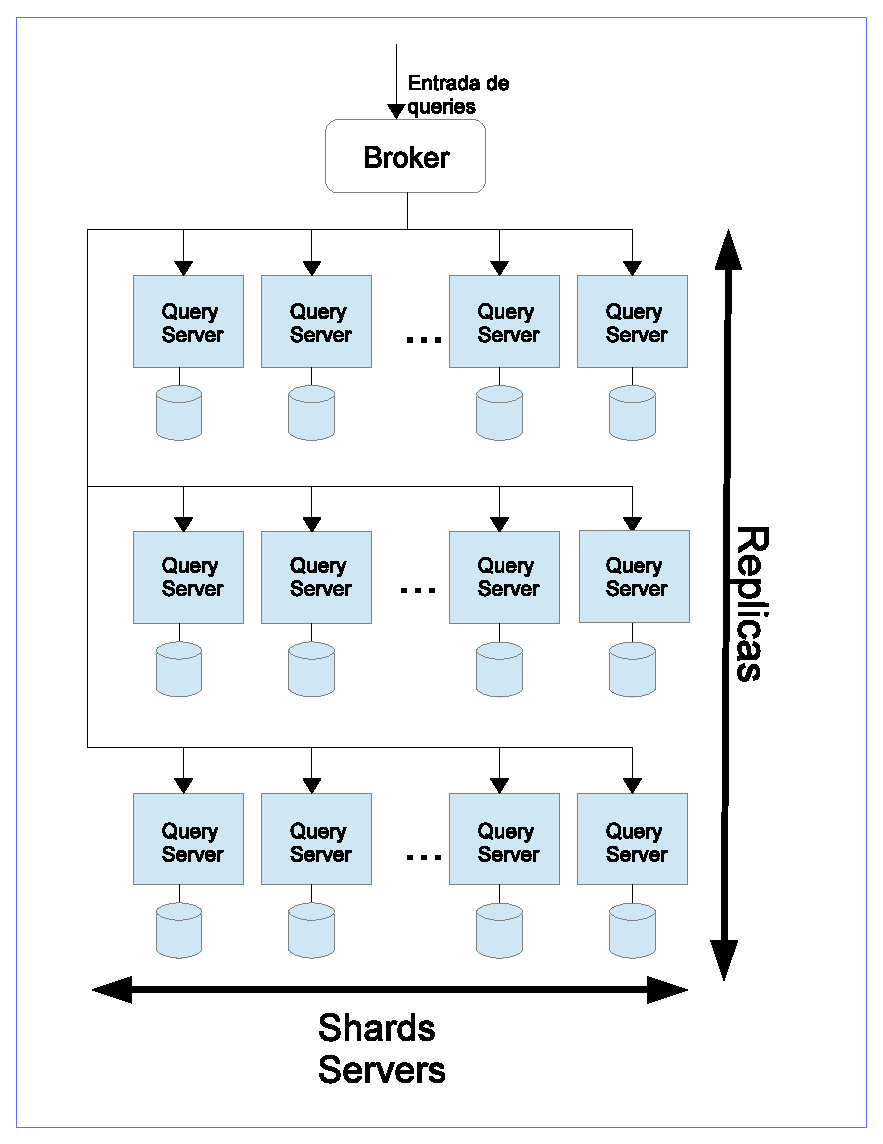
\includegraphics[scale=.75]{images/sistemaIR.eps}
\caption{Arquitectura de un sistema de recuperación de la información con réplicas}
\label{fig:sistemaIR}
\end{figure}

\subsection{Trabajo relacionado}
\label{marco:tr}
El estudio \citep{Broccolo:2013} analiza métodos de \textit{dropping} y \textit{stopping} para el procesamiento de consultas bajo altas carga de trabajo en un sistema distribuído donde existen múltiples servidores en el que cada uno resuelve una parte de la consulta para luego enviar las consultas al \textit{broker} y éste hace el \textit{merge} de los resultados de acuerdo al \textit{score} de los documentos. Se define un tiempo \textit{T}, en el que la suma de el tiempo de espera de la consulta para ser procesada ($t_{w}$) y el tiempo de procesamiento de la misma ($t_{p}$) deben ser menor a \textit{T}. Si es que se sobrepasa este tiempo, se tienen dos opciones (1) la consulta es desechada y se envía al \textit{broker} una lista vacía, (2) se detiene el procesamiento de la transacción de lectura y se envía los resultados parciales hasta el momento. Finalmente se propone un método basado en la predicción de tiempo de respuesta ($\hat{pt}(q)$) de una consulta \citep{Macdonald:2012} de modo que si se cumple $ \hat{pt}(q) \leq T - wt(q) $, entonces la consuta es desechada antes de comenzar a procesarse y se toma la siguiente desde la cola de espera. Notar que en estos métodos existe una pérdida de efectividad, puesto que eventualmente los servidores muchas veces no enviarán sus mejores documentos al \textit{broker}, esto implica que el \textit{broker} responderá al usuario un conjunto de K documento que no necesariamente son los mejores dentro del corpus completo.

En \citep{Freire:2012} se estudia el impacto que tiene la técnica de predicción de tiempos de respuestas para consultas, \citep{Tonellotto:2011} en sistemas de recuperación de la información con réplicas. En este estudio, se llega a la conclusión que usando una buena predicción, se puede reducir el tiempo que la consulta tiene que esperar para ser procesada ($t_{w}$), y también se puede reducir el tiempo total requerido para procesar el conjunto (\textit{log}) completo de transacciones de lectura (\textit{completion time}). En \citep{Freire:2013}, se propone un modelo híbrido de \textit{scheduling} de consultas a través de réplicas, en el que cuando el sistema se encuentre bajo altas cargas de trabajo, se utilice política de \textit{scheduling} basada en la predicción de tiempo de respuesta de las consultas \citep{Macdonald:2012} y cuando el sistema se encuentre con una baja carga de trabajo, se utilice una politica de \textit{scheduling} sencilla y de menor costo como \textit{Round Robin}.